\documentclass[11pt,a4paper]{article}
\usepackage[margin=2.3cm,headheight=14pt]{geometry}
\usepackage{lmodern}
\usepackage[T1]{fontenc}
\usepackage{amsmath,amssymb,bm}
\usepackage{booktabs,array,tabularx}
\usepackage{graphicx}
\usepackage[dvipsnames]{xcolor}
\usepackage[skins,breakable]{tcolorbox}
\usepackage{caption}
\usepackage{float}
\usepackage{fancyhdr}
\usepackage{enumitem}
\usepackage{siunitx}
\usepackage{microtype}
\usepackage[colorlinks=true,linkcolor=NavyBlue,citecolor=NavyBlue,urlcolor=NavyBlue]{hyperref}

\sisetup{per-mode=symbol,detect-all}
\captionsetup{font=small,labelfont=bf}
\setlength{\parskip}{0.45em}
\setlength{\parindent}{0pt}
\numberwithin{equation}{section}
\definecolor{note}{HTML}{1F4E79}
\definecolor{keybg}{HTML}{F3F7FB}
\newtcolorbox{keyresult}{enhanced,colback=keybg,colframe=note!60,boxrule=0.6pt,arc=2pt,
  left=8pt,right=8pt,top=4pt,bottom=4pt}
\newtcolorbox{remark}[1][Remark]{enhanced,breakable,colback=note!4,colframe=note,
  boxrule=0pt,leftrule=3pt,arc=0pt,left=6pt,right=6pt,top=4pt,bottom=4pt,
  title={\textbf{#1}},coltitle=note,colbacktitle=note!4,attach title to upper={\ \ },fonttitle=\small}
\graphicspath{{figures/}}

\pagestyle{fancy}
\fancyhf{}
\fancyhead[L]{\small Eccentric-cavity soft bending actuator}
\fancyhead[R]{\small Grasp analysis}
\fancyfoot[C]{\small\thepage}
\renewcommand{\headrulewidth}{0.4pt}

\begin{document}

\begin{center}
{\LARGE\bfseries How much can the fingers lift?\par}
\vspace{4pt}
{\large Grasp model for tapered, curling pneumatic fingers with frictional contact\par}
\vspace{6pt}
{\small Rudranarayan Pradhan \quad\textperiodcentered\quad October 2026}
\end{center}

\section{Question}
The actuator should curl, at least over part of its length, into a hook or spiral that can close round an
object. The question asked here is: \emph{for a given friction coefficient $\mu$ between finger and object,
how large an upward force can the curled fingers exert on a rigid object before it slips out?}
The answer is read directly from the contact reaction forces that the (rigid) object exerts on the fingers.

\section{Model}

\subsection{Finger}
Each finger is a silicone tube with a hoop-thread winding (so it cannot balloon) and an inextensible
strain-limiting layer along the side that faces the object. The layer pins the neutral axis, so the finger is
an inextensible planar rod whose reference line is the layer, which is also the contact surface.
Cut the finger at arc length $s$ and keep the tip piece together with the air inside it: the air beyond the
cut pushes with $P\pi r(s)^2$ through the cavity centre, a lever $d(s)$ from the layer. Moment balance gives
\begin{equation}
m(s) = EI(s)\,\big[\kappa(s)-\kappa_0(s)\big],\qquad
\kappa_0(s) = \frac{P\,\pi r(s)^2\,d(s)}{EI(s)},
\label{eq:kappa0}
\end{equation}
where $m$ is the moment of the contact forces beyond $s$ and $EI$ is the bending stiffness about the layer.
Pressure therefore acts as a \emph{spontaneous curvature} $\kappa_0$, and contact forces bend the finger
away from it. For a concentric cavity of radius $r=R-t$ in a tube of outer radius $R$ and wall $t$, with the
layer on the outer surface ($d=R$),
\begin{equation}
I = \tfrac{\pi}{4}(R^4-r^4) + \pi(R^2-r^2)R^2,\qquad
\kappa_0 \;\xrightarrow{\;t\ll R\;}\; \frac{P}{3\,E\,t}.
\label{eq:thin}
\end{equation}

\begin{keyresult}
\textbf{The wall thickness, not the outer radius, sets how tightly a section curls.}
Tapering only the outer radius leaves $\kappa_0$ almost unchanged and mainly softens the tip. To make the tip
curl more tightly than the base, the wall must thin toward the tip as well; alternatively, the
strain-limiting layer can be placed only on the distal part, so that only the tip curls.
\end{keyresult}

\subsection{Designs compared}
All fingers are \SI{100}{mm} long, $E=\SI{0.15}{MPa}$ (a soft silicone such as Dragon Skin 10), with a hoop
winding and a concentric cavity.
\begin{center}\small
\begin{tabular}{@{}lll@{}}
\toprule
Design & Section & Layer\\
\midrule
uniform  & $R=\SI{10}{mm}$, $t=\SI{2}{mm}$ & full length\\
tapered  & $R$: \SIrange{10}{5}{mm}, $t$: \SIrange{2}{1}{mm} (scaled copy) & full length\\
tip-hook & $R=\SI{10}{mm}$, $t=\SI{2}{mm}$ & last \SI{40}{\percent} only\\
\bottomrule
\end{tabular}
\end{center}
In the tapered finger the section shrinks in proportion, so $\kappa_0\propto 1/R$ and the tip curls twice as
tightly as the base, giving a spiral (Figure~\ref{fig:shapes}).

\begin{figure}[H]
\centering
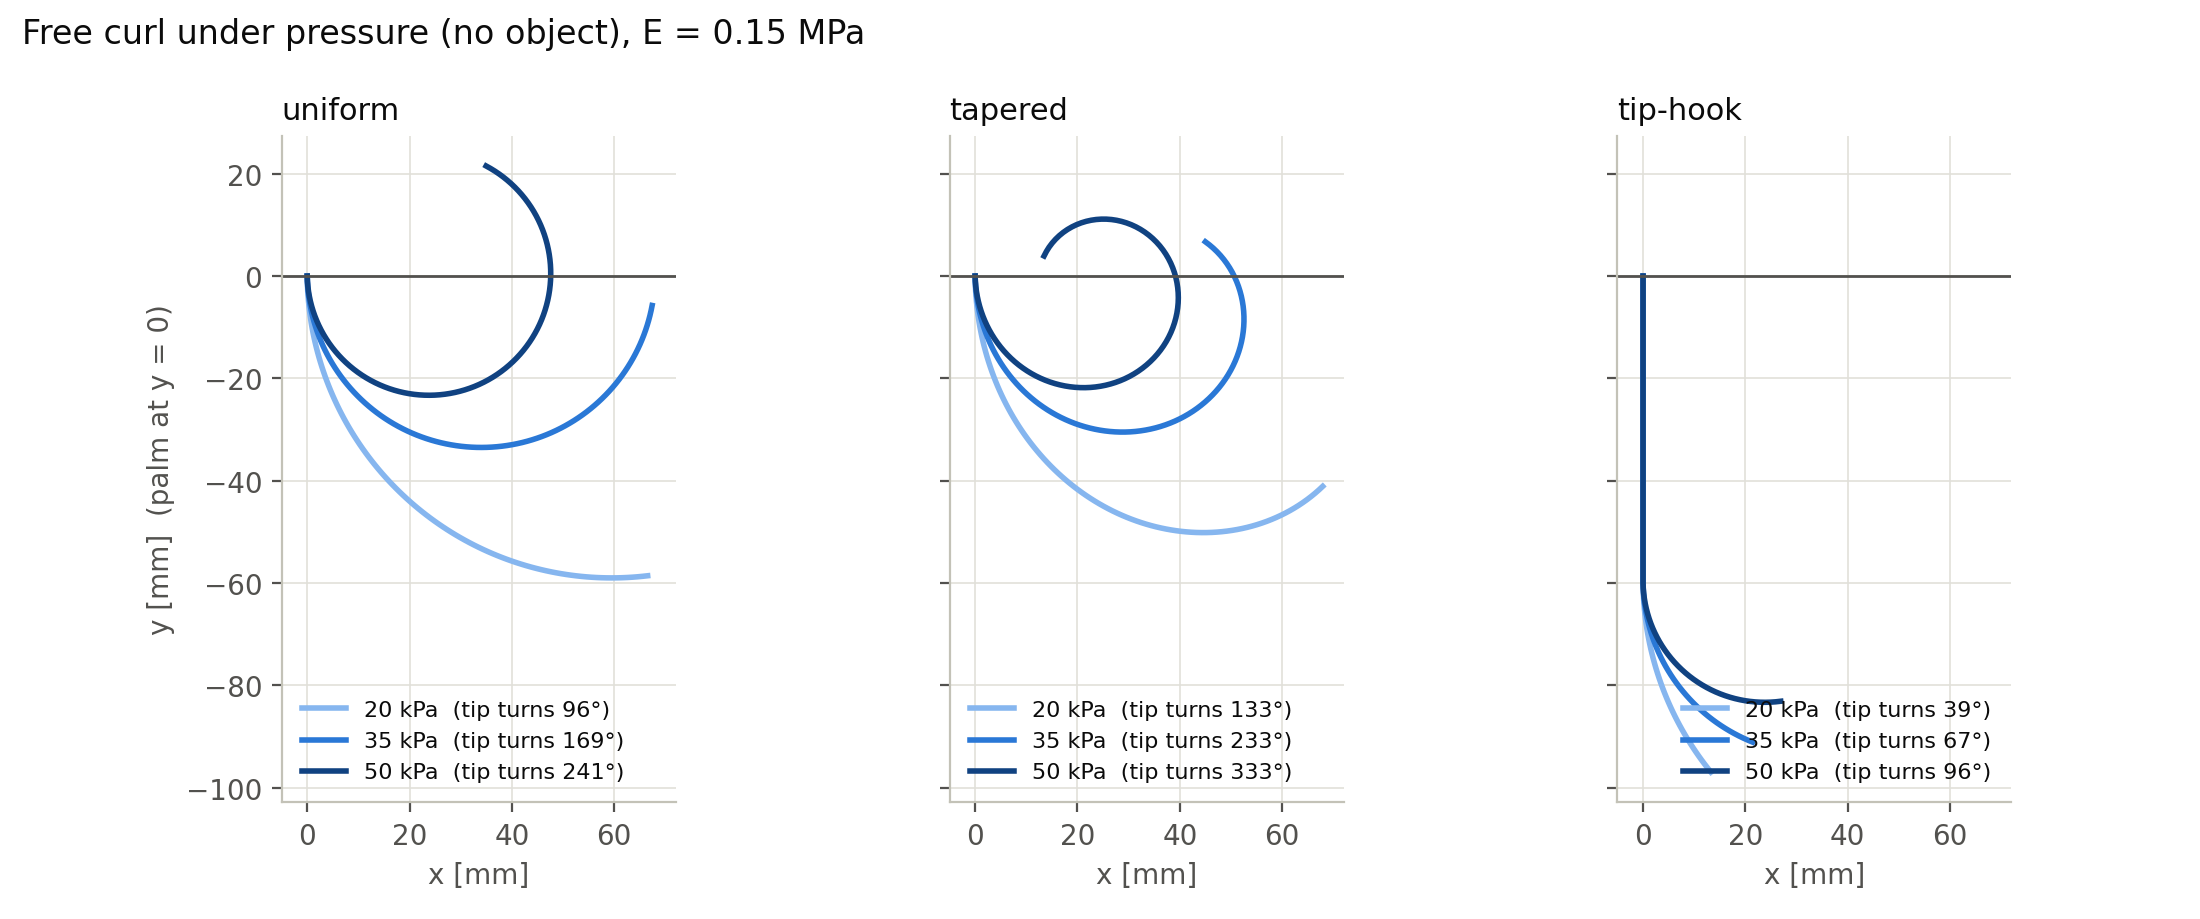
\includegraphics[width=\textwidth]{grasp_shapes.png}
\caption{Free curl (no object) at three pressures. Uniform: circular arc. Tapered: tightening spiral.
Tip-hook: straight base, curled tip.}
\label{fig:shapes}
\end{figure}

\subsection{Grasp}
Two mirrored fingers hang from a palm at $y=0$, the layers \SI{1}{mm} from a rigid cylinder of radius
$a=\SI{15}{mm}$ whose centre lies on the axis at depth $h$ below the palm. By symmetry only the left finger
is solved; the plane $x=0$ acts as a frictionless wall where the two fingertips may meet beneath the object.

\textbf{Contact.} Each rod node $\bm p_i$ is pushed out of the cylinder by a penalty force
$F_{n,i}=k_n\langle a-|\bm p_i-\bm c|\rangle$. Friction follows Coulomb's law with stick and slip: each contact
node carries an anchor $\xi_i$ on the object surface, a tangential spring $k_t(u_i-\xi_i)$ acts while it sticks,
and the anchor slides when the spring force would exceed $\mu F_{n,i}$. Within a load step this is the convex,
continuously differentiable potential
\begin{equation}
\psi_i = \begin{cases} \tfrac12 k_t\,\delta_i^2, & |\delta_i|\le \mu F_{n,i}/k_t\\[2pt]
\mu F_{n,i}\big(|\delta_i| - \tfrac{\mu F_{n,i}}{2k_t}\big), & \text{otherwise,}\end{cases}
\qquad \delta_i = u_i-\xi_i ,
\end{equation}
with $F_{n,i}$ updated by fixed-point iteration until it changes by less than \SI{e-5}{N}.

\textbf{Loading.} (1) The pressure rises from 0 to $P$ with the object held still, so the fingers close on it.
(2) The object is then pulled down in steps (displacement control). At every step the force the fingers exert
on the object is obtained from the contact potentials, $\bm F = -\partial(U_n+\Psi)/\partial\bm c$, and split
into its normal and friction parts. Doubling the vertical component (two fingers) gives the upward force on the
object; its maximum over the pull is the \textbf{holding capacity}, i.e.\ the largest weight the grasp can carry.

\textbf{Solution.} 100 rod segments; for each step the total potential (bending, contact, friction) is minimised
with a trust-region Newton method using exact gradients and Hessians from JAX
(\texttt{grasp\_model.py}). One grasp, inflation plus pull, takes about \SI{2}{s}.

\subsection{Checks}
\begin{itemize}[nosep]
\item Free curl: the solver reproduces the closed-form integral of $\kappa_0$ to machine precision
(tip angle \ang{192.64} at \SI{40}{kPa}, tip position error \SI{e-13}{mm}).
\item Force consistency (frictionless): the reaction force summed from the contacts equals the derivative of the
stored energy with respect to the object position, computed by finite differences.
\item Numerical parameters: doubling the contact stiffness changes the holding force by \SI{0.1}{\percent};
refining the rod from 100 to 160 segments changes it by \SI{0.35}{\percent}.
\item Convergence: every step solves to a gradient below \num{e-9}. The friction--normal-force coupling is
iterated with under-relaxation; in 379 of 420 runs every step closes to below \SI{e-3}{N}. The remaining steps all
lie in the final slip-out at high friction, well after the holding force is reached (residual at the peak
$\le\SI{3e-3}{N}$), and the peaks agree with an independent first pass to within \SI{0.01}{N}.
\end{itemize}

\section{How the holding force is measured}
The object is pulled down from the position where it was grasped. Two numbers are read from the force curve:
\begin{description}[nosep,leftmargin=1.5em]
\item[Working holding force] the largest upward force reached within \SI{10}{mm} of sag. This is the weight the
grasp carries without the object dropping noticeably, and it is the design number.
\item[Ultimate pull-out force] the peak over the whole pull, which may need the object to drop by several
centimetres first. It relies on the strain-limiting layer being perfectly inextensible and is an upper bound.
\end{description}

\begin{figure}[H]
\centering
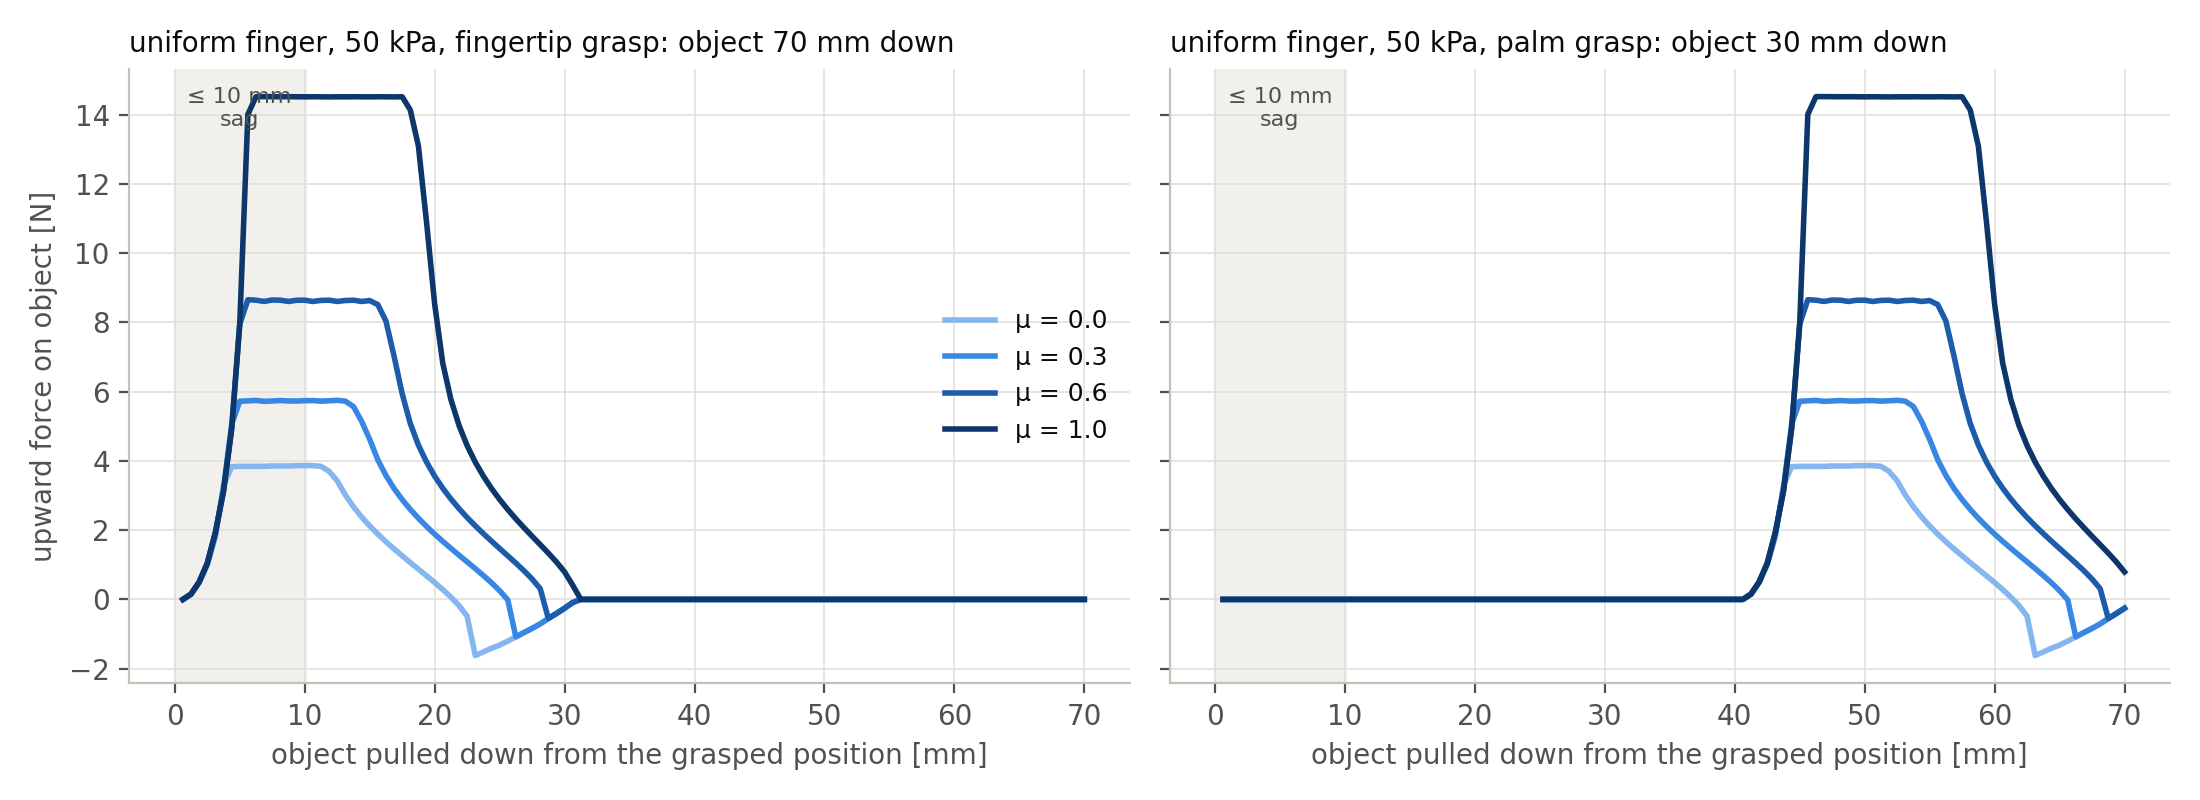
\includegraphics[width=\textwidth]{grasp_curves.png}
\caption{Upward force on the object as it is pulled down, uniform finger at \SI{50}{kPa}. Left: object near the
fingertips; the tips are already under it and the force rises to its plateau within \SI{6}{mm}. Right: object near
the palm; it hangs loose in the closed fingers and drops \SI{40}{mm} before the tips catch it. The plateau is the
hooked fingertips sliding round the object at the friction limit; the shaded band is the \SI{10}{mm} sag window.}
\label{fig:curves}
\end{figure}

\section{Results}
The sweep covers the three designs, object depths \SIrange{20}{80}{mm} (step \SI{10}{mm}), pressures
\SIrange{10}{50}{kPa} and $\mu = 0,\,0.3,\,0.6,\,1.0$: 420 grasps (\texttt{grasp\_study.py}).

\begin{figure}[H]
\centering
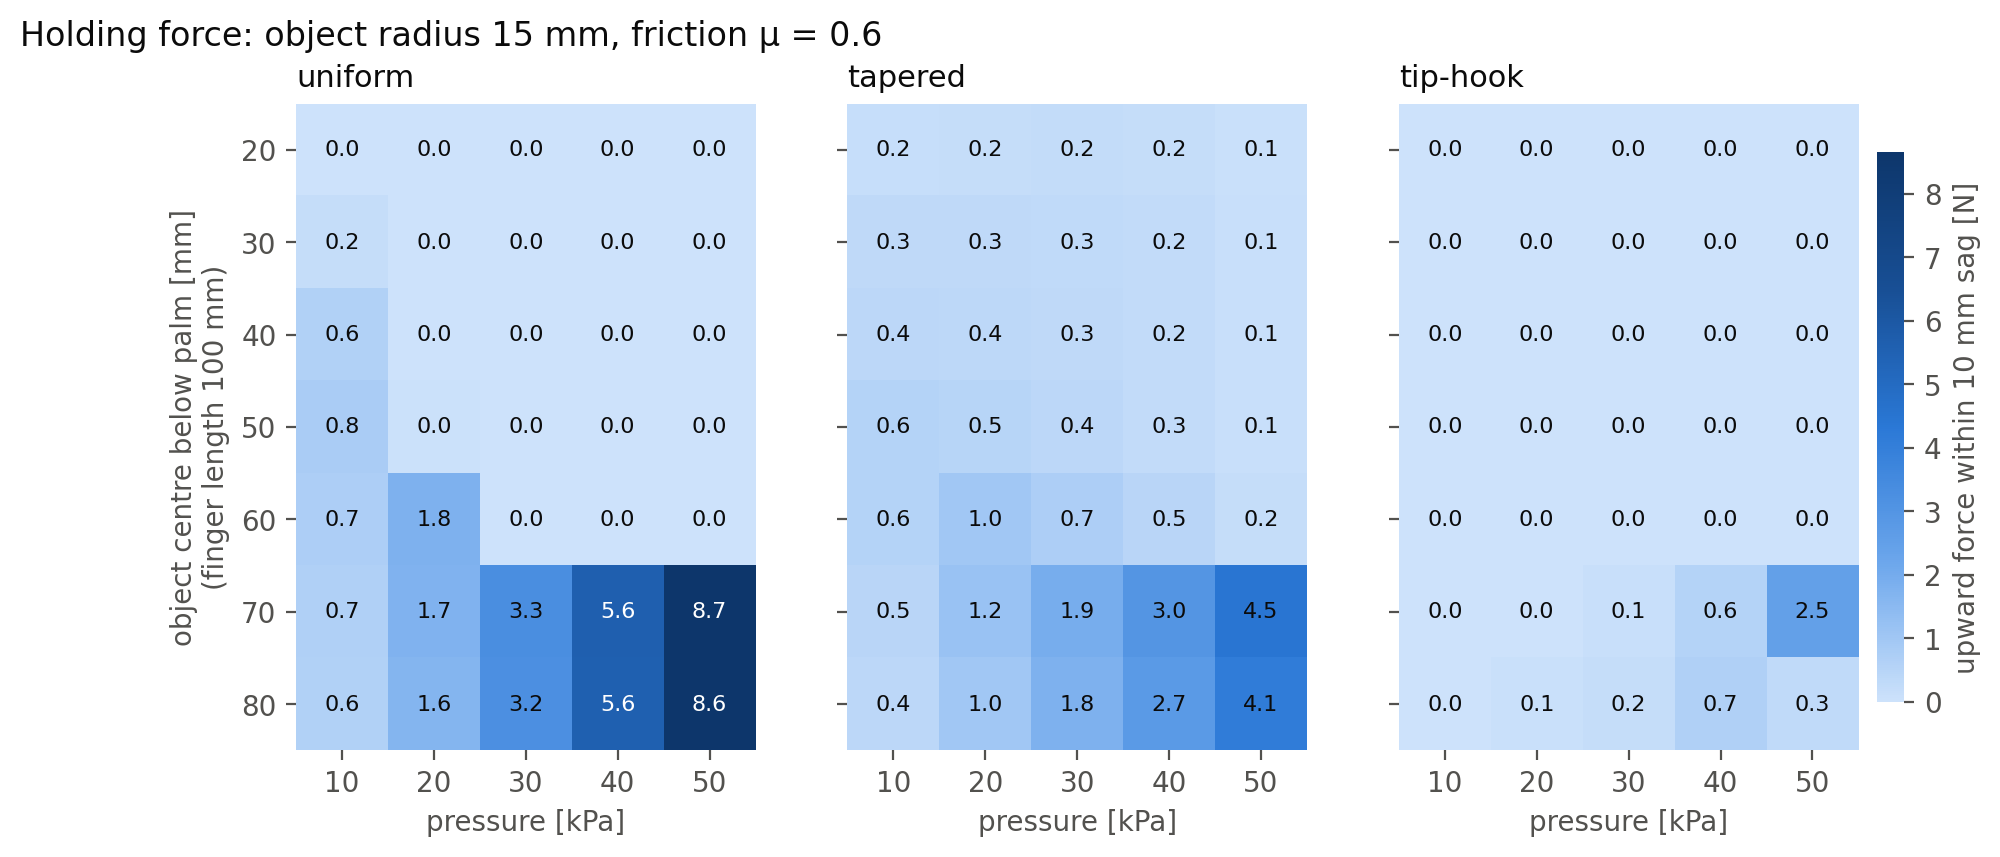
\includegraphics[width=\textwidth]{grasp_maps.png}
\caption{Working holding force against object depth and pressure, $\mu=0.6$. Only objects near the fingertips are
held firmly; objects near the palm are caged loosely and give no force within \SI{10}{mm} of sag.}
\label{fig:maps}
\end{figure}

\begin{figure}[H]
\centering
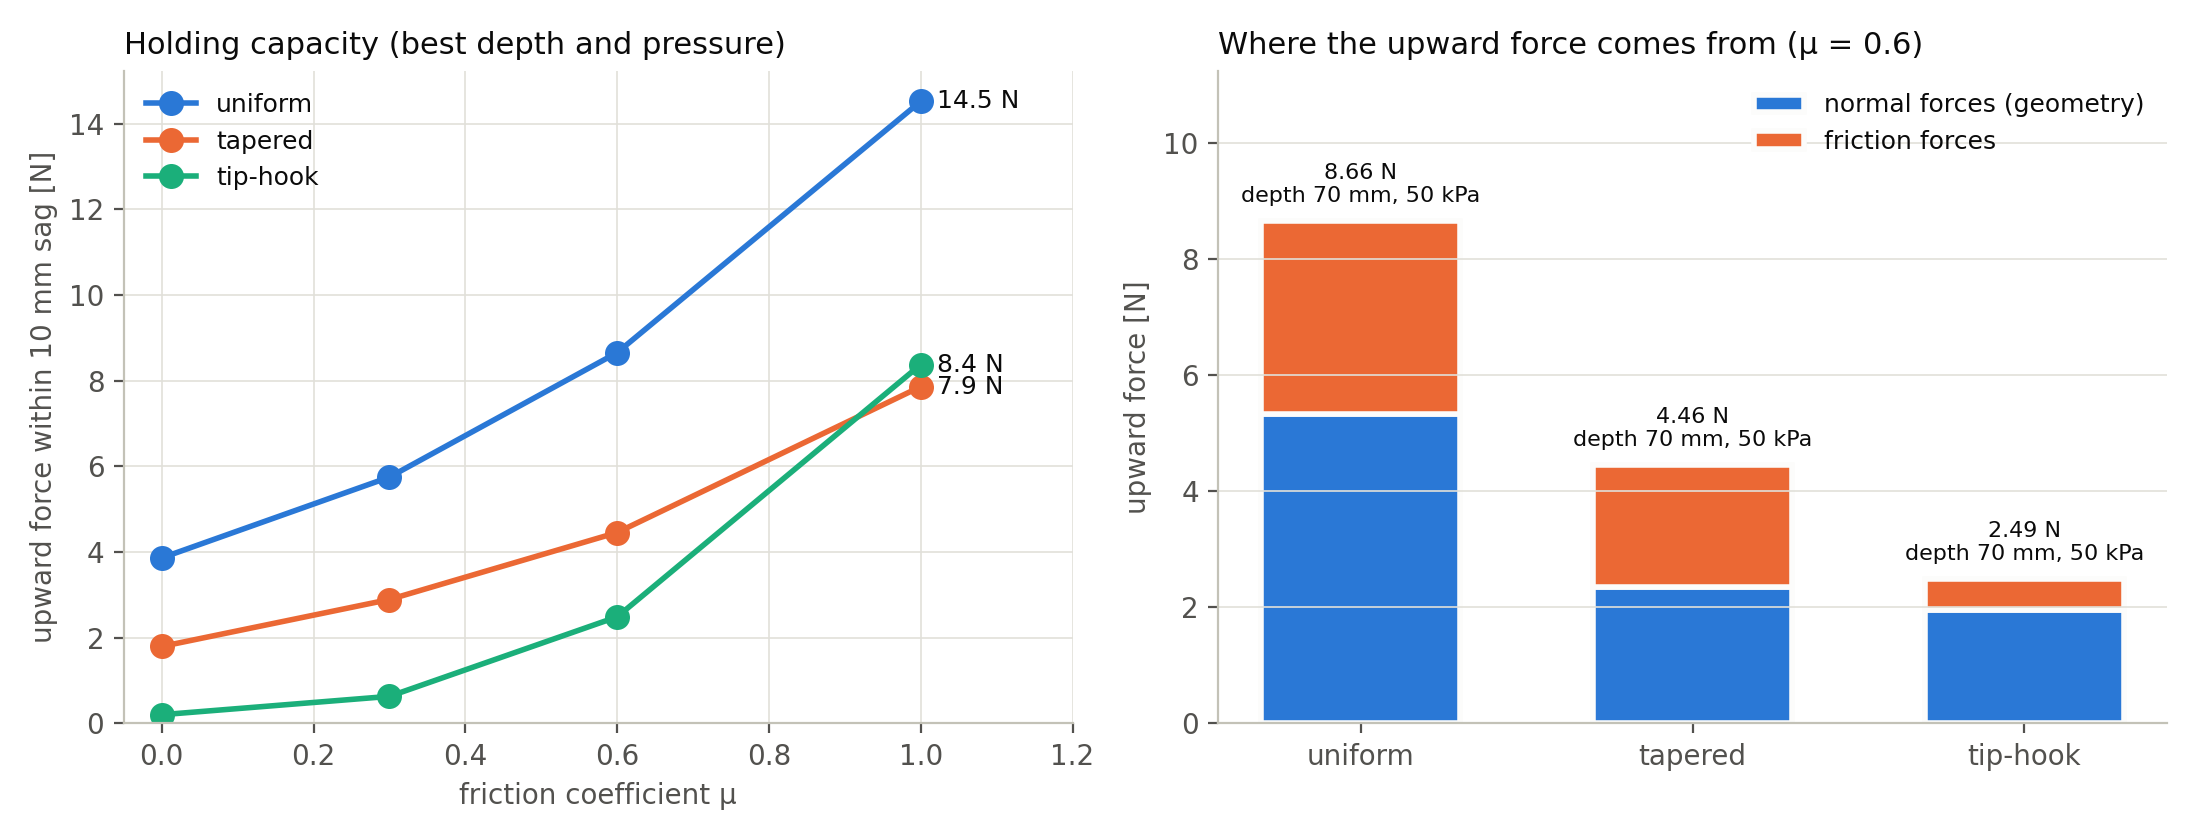
\includegraphics[width=\textwidth]{grasp_capacity.png}
\caption{Left: best working holding force against friction. Right: its split into the vertical components of the
normal and the friction contact forces at $\mu=0.6$.}
\label{fig:capacity}
\end{figure}

\begin{table}[H]
\centering\small
\begin{tabular}{@{}lcccc@{}}
\toprule
& \multicolumn{4}{c}{holding force [N]}\\
\cmidrule(l){2-5}
Design & $\mu=0$ & $\mu=0.3$ & $\mu=0.6$ & $\mu=1.0$\\
\midrule
uniform  & 3.87 & 5.75 & 8.66 & 14.53\\
tapered  & 1.80 & 2.89 & 4.46 & 7.86\\
tip-hook & 0.20 & 0.63 & 2.49 & 8.38\\
\bottomrule
\end{tabular}
\caption{Best working holding force (two fingers, \SI{50}{kPa}, object \SIrange{70}{80}{mm} below the palm).
With the object near the fingertips the ultimate pull-out force equals the working force, because the plateau is
reached within \SI{10}{mm}.}
\label{tab:capacity}
\end{table}

\begin{figure}[H]
\centering
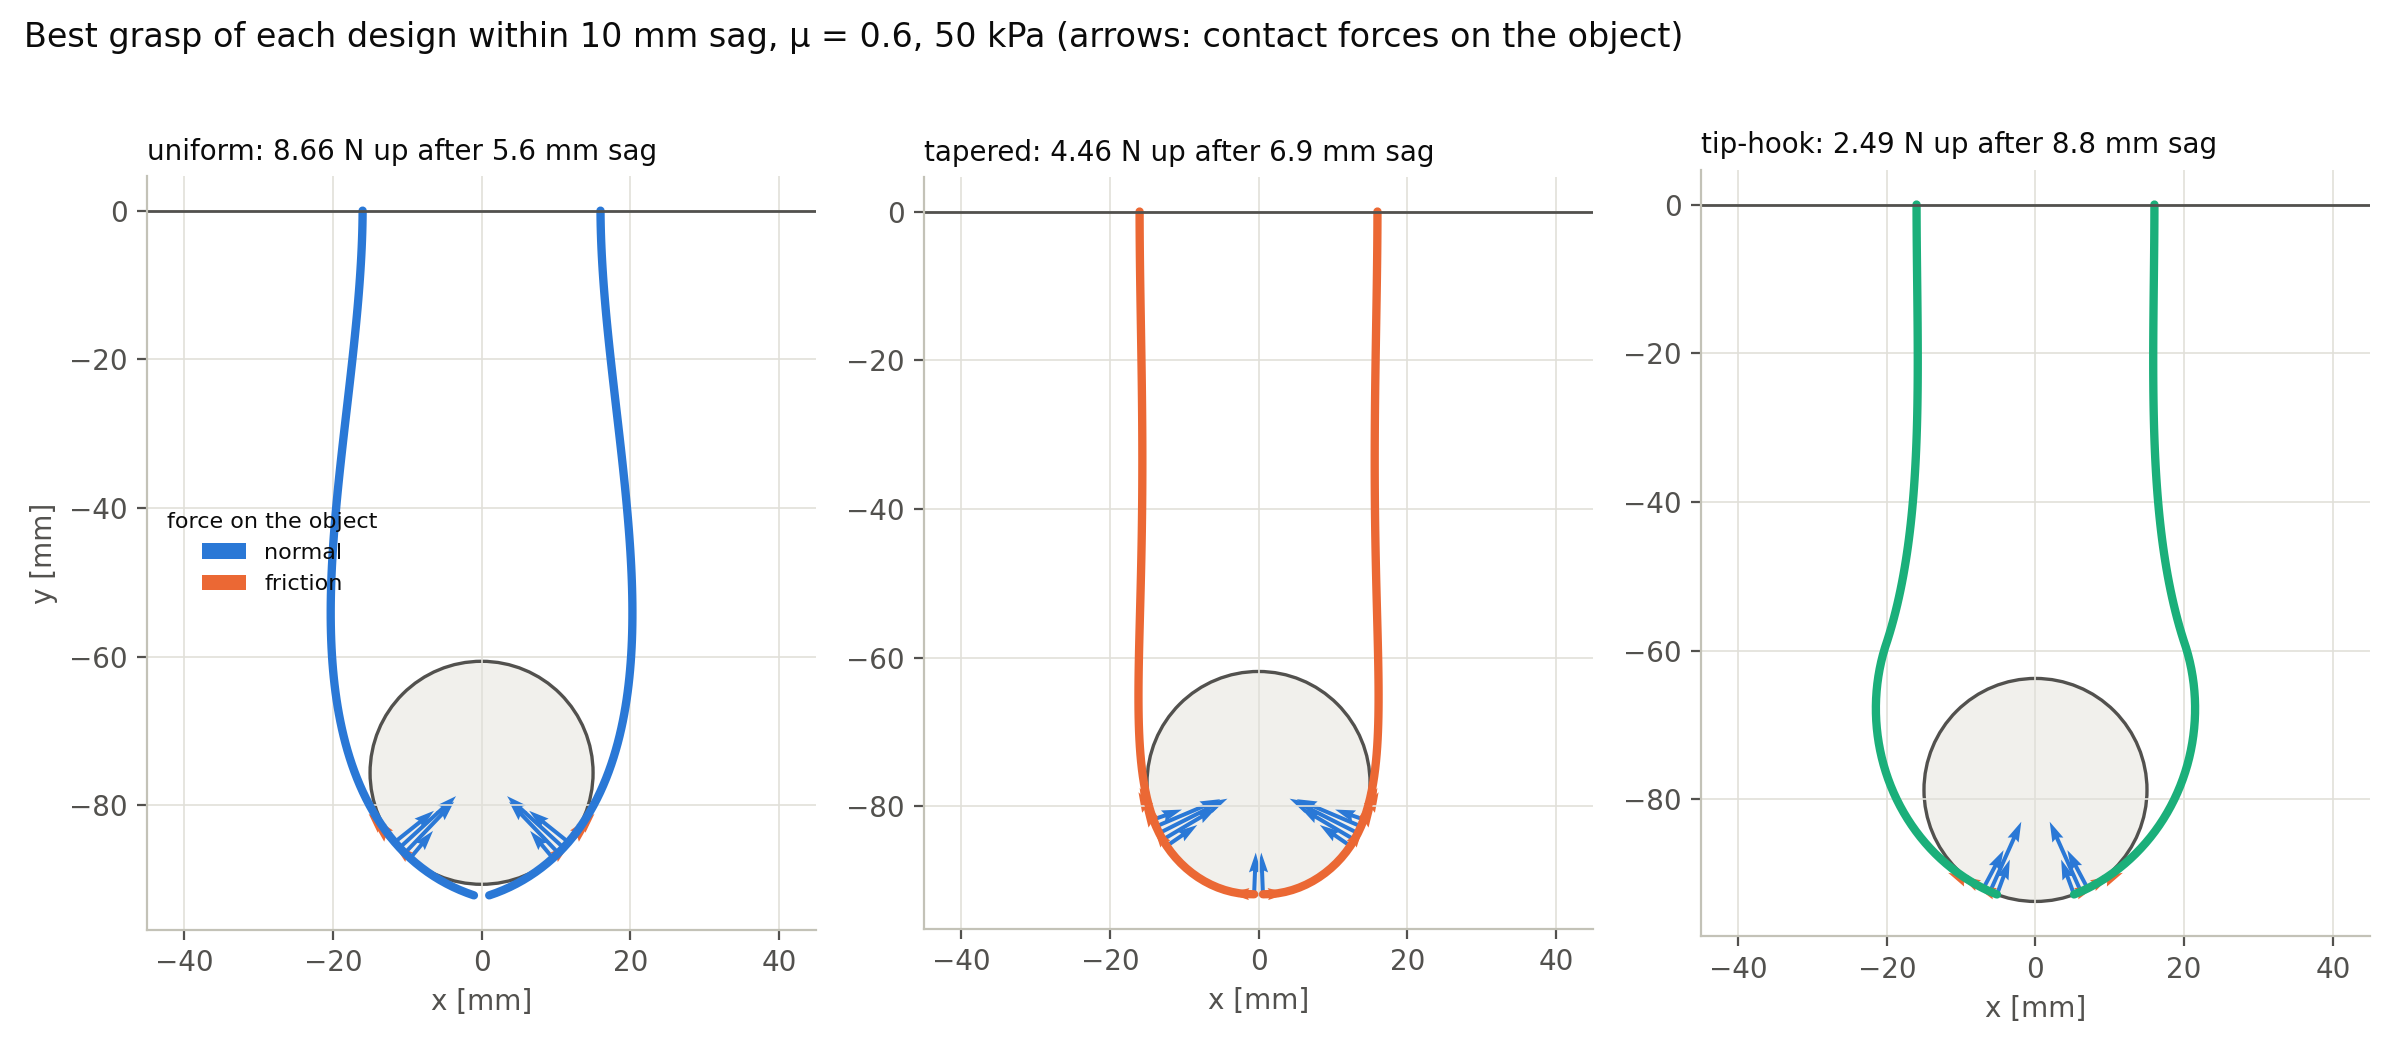
\includegraphics[width=\textwidth]{grasp_snapshots.png}
\caption{Best grasp of each design at the working holding force, $\mu=0.6$. Arrows: contact forces on the object.
The fingertips curl under the object; nearly all of the upward force acts on its lower third.}
\label{fig:snap}
\end{figure}

\begin{enumerate}
\item \textbf{Grasp near the fingertips, not near the palm.} The firm grasp is a \emph{fingertip hook}: the object
sits where the fingers curl, roughly \SIrange{70}{80}{\percent} of the finger length below the palm, and the curled
tips are already under it. An object near the palm hangs loose in the closed fingers (they meet beneath it) and
drops \SIrange{40}{50}{mm} before the tips catch it (Figure~\ref{fig:curves}, right).
\item \textbf{Friction roughly doubles to quadruples the grip.} For the uniform finger the working force rises from
\SI{3.9}{N} at $\mu=0$ to \SI{8.7}{N} at $\mu=0.6$ and \SI{14.5}{N} at $\mu=1$; at $\mu\ge0.6$ friction supplies
more than a third to over half of the upward force (Figure~\ref{fig:capacity}). A tacky or textured contact
surface is the cheapest way to lift more.
\item \textbf{Pressure helps more than linearly.} At the best depth the uniform finger holds 0.7, 1.7, 3.3, 5.6 and
\SI{8.7}{N} at 10--\SI{50}{kPa} ($\mu=0.6$): both the curl and the stiffness of the curled tip grow with pressure.
\item \textbf{Tapering the outer radius halves the grip.} The tapered finger curls into a tighter spiral but its tip
is $2^4=16$ times less stiff, so the hook opens under a smaller load: \SI{4.5}{N} against \SI{8.7}{N} at
$\mu=0.6$. A taper is useful for wrapping objects of different sizes, not for holding force.
\item \textbf{A short tip hook is weak unless friction is high.} With the layer on only the last \SI{40}{mm}
the hook turns about \ang{96} at \SI{50}{kPa}, too little to get under a \SI{30}{mm} object; it relies on friction
(\SI{0.2}{N} at $\mu=0$, \SI{8.4}{N} at $\mu=1$). A thinner wall in the hook would let it curl further.
\end{enumerate}

\section{Segmented fingers}
A finger with $n$ sealed chambers in series, each fed separately, has a piecewise-constant spontaneous curvature:
a cut inside chamber $k$ sees only $P_k$, so the finger bends only where its chambers are inflated. The model
takes one pressure per chamber (\texttt{Finger(n\_seg=4)}, \texttt{step(P=[P1, P2, P3, P4])}). Inflating single
chambers places the bend anywhere along the finger, adjacent chambers make a hook or a spiral, and inflating them
in sequence moves the bend from base to tip (animation \texttt{report/animations/tentacle\_segments}).

Four chambers of \SI{25}{mm}, wall \SI{1.5}{mm}, \SI{50}{kPa}: the free finger curls \ang{348}. With the object near
the fingertips this finger holds \SI{14.2}{N} at $\mu=0.6$, against \SI{8.7}{N} for the uniform \SI{2}{mm}-wall finger:
the thinner wall curls more tightly and hooks further under the object.

\textbf{Inflation order} (\texttt{grasp\_sequence.py}). Inflating all chambers together, base to tip, or tip to base
gives the same grip to within \SI{0.2}{\percent} in almost every case, \emph{except} when the object sits at the
fingertips: inflating the tip first curls the tip before the finger has closed and it ends up outside the object
(\SI{0}{N}). Inflate from the base, or all together. The animation \texttt{tentacle\_grasp} shows a base-to-tip grasp
and the pull-out.

\section{Limitations}
\begin{itemize}[nosep]
\item Planar model of a cylindrical object with two mirrored fingers; no out-of-plane wrapping, no palm contact,
no friction between the fingertips where they meet.
\item Linear beam law with a perfectly inextensible strain-limiting layer and a perfect hoop winding (no
ballooning). Beyond a curl of about half a turn the strains are large and the 3-D FE model should be used to
confirm the numbers.
\item Rigid object, point-wise penalty contact on the layer line; finger self-weight is neglected
(about \SI{0.1}{N} per finger, small next to the holding forces).
\end{itemize}

\section{Next steps}
\begin{enumerate}[nosep]
\item Measure $\mu$ between the cured silicone and typical objects (inclined-plane test) and the silicone's $E$.
\item Check the best fingertip grasp with the 3-D FE model (add the strain-limiting layer and contact) and in ANSYS.
\item Build one segmented finger; test the holding force by hanging weights from a grasped cylinder and compare
with Table~\ref{tab:capacity}.
\end{enumerate}

\textbf{Code:} \texttt{grasp\_model.py} (model), \texttt{grasp\_study.py} (sweep), \texttt{grasp\_sequence.py}
(inflation order), \texttt{grasp\_figures.py} (figures), \texttt{tentacle\_animation.py} (animations).

\end{document}
